\documentclass{llncs2e/llncs}
%
\usepackage{makeidx}  % allows for indexgeneration
\usepackage{graphicx}
\usepackage{amssymb}
\usepackage{amsmath}
\usepackage{listings}
\usepackage{pgf,tikz}
\usepackage{float}
\usepackage{ulem}
\usetikzlibrary{arrows}
\usetikzlibrary{positioning,shapes,fit}
\usepackage{xcolor, color, colortbl}
\usepackage{tikz-qtree}
\usepackage{subcaption}
\captionsetup{compatibility=false}
%
\begin{document}
%
\pagestyle{headings}  % switches on printing of running heads
%
\title{Implementing a C Memory Model Supporting Integer-Pointer Casts in CompCert}
%
\titlerunning{Integer-Pointer Casts Semantics in CompCert}  % abbreviated title (for running head)
\author{Aur\`ele Barri\`ere}
%
\authorrunning{Aur\`ele Barri\`ere} % abbreviated author list (for running head)
%
\institute{\'Ecole Normale Sup\'erieure de Rennes, France\\
\email{aurele.barriere@ens-rennes.fr}\\ 
}

\maketitle              % typeset the title of the contribution

\hrulefill

\begin{center}
  \textbf{Supervisor: } Professor Chung-Kil Hur\\
  Software Foundations Laboratory\\
  Seoul National University, South Korea
\end{center}

\hrulefill

\begin{center}
  \textbf{May 15 2017 - August 4 2017}
\end{center}

\vfill
\begin{center}
\includegraphics[width=4cm]{img/enslogo.png}
\quad\quad\quad
\includegraphics[width=4cm]{img/snulogo.png}
\end{center}
\vfill
\begin{abstract}
  The ISO standard for the C programming language does not define semantics for integer-pointer casts. The certified C compiler CompCert uses an abstract memory model which allows for many optimizations, but in which the behavior of such casts is undefined. In~\cite{DBLP:conf/pldi/KangHMGZV15}, Kang et al. present a formal memory model that supports integer-pointer casts semantics, while still allowing common optimizations.
  We show the relevance of this model by implementing both the memory model and the cast semantics in CompCert. We present the changes that need to be done, both in the way CompCert transforms C programs and in the proofs.
\keywords{CompCert, C Memory Model, Integer-Pointer Cast, Optimization}
\end{abstract}
%
\newpage

\def\todo#1{{\color{red}TODO:\quad#1}}
\def\addref#1{{\color{red}$[$#1$]$}}
\def\undef{\textit{undef}}
\def\states#1{\mathit{States_{#1}}}
\def\step#1{\mathit{Step_{#1}}}
\def\atstep#1{\mathit{AtomicStep_{#1}}}
\def\traces{\mathit{Traces}}

\section{Introduction}
When compiling critical software written in C, one expects from the compiler to not introduce any bugs, or any behavior that wasn't specified in the C source code.%
% compcert and coq
To meet this expectation, CompCert~\cite{DBLP:journals/cacm/Leroy09} is a formally verified C compiler.
It uses the Coq Proof Assistant~\cite{coq} to prove that the compiled code and the source code have the same observable behavior, as defined by the ISO C Standard~\cite{iso}.
CompCert also aims to provide performance of the generated code, and implements several common optimizations. Compiled code runs approximately 10\% slower than code compiled with \texttt{GCC4 -O1}~\cite{compcertwebsite}.
As of today, CompCert is a trusted compiler; despite many efforts~\cite{DBLP:conf/pldi/YangCER11}, no bug have been discovered within the verified parts of CompCert.
CompCert currently supports all of the ISO C 99 Standard, with very few exceptions~\cite{compcertwebsite}.

% iso c and semantics
However, the ISO C standard itself does not define semantics for every syntactically valid C program.
Many C programs are said to have \textit{unspecified behavior} or \textit{undefined behavior}, meaning that conforming compilers can produce any compiled code.
Despite the lack of semantics, many C programmers are using such programs and expect a precise result. %not a very good sentence
This leads to difficult bugs~\cite{DBLP:conf/apsys/WangCCJZK12} and the impossibility of proving that the compiled code behaves as expected.

% integer pointer casts
One popular unspecified feature of the C language is the casting between integer and pointer values.
Such casts have many uses in real C programs. For instance, pointer to integer cast is used in the Linux Kernel or JVM implementations for bitwise operations on pointers. Integer arithmetic on pointers is used in Linux, FreeBSD, QEMU and others~\cite{cerberus}. Another common usage is to use the bit represenation of a pointer as indexing key of a hash table (used for instance in the C++ standard library).
When compiled with most compilers, those programs behave as expected from the programmers. But these intuitive semantics have not been formalized in the C standard.

% motivation of the Kanget al. paper
Defining a precise, formal semantics for integer-pointer casting and pointer manipulation would allow CompCert to compile even more C programs in a certified way.
The semantics of pointer manipulation depends on the memory model of the compiler.
As of today, CompCert uses a logical memory model~\cite{leroy:hal-00703441}, where every memory block is an abstract object without a concrete memory address. Such a memory model enables many optimizations, because a program can never guess the location of a block and modify it without a pointer (see section~\ref{sec:prelim}).
However, integer-pointer casting isn't possible.
Other works have investigated the use of a concrete memory model, to reflect the memory state of a real machine~\cite{DBLP:conf/popl/TuchKN07}\cite{Norrish98cformalised}. But then, most optimizations cannot be done anymore without changing the behavior of the program.

In~\cite{DBLP:conf/pldi/KangHMGZV15}, Kang et al suggest a quasi-concrete model, in which there are both logical and concrete memory blocks. The main idea is to use logical blocks by default, that can allow optimizations, and use concrete blocks when the concrete address of a memory block is needed.

% contribution
We implemented this new memory model in CompCert.
In this paper, we discuss this implementation.
We show that it is relevant and supports integer-pointer casts while still allowing common optimizations.
We present the difficulties of the implementation, and the changes that needed to be done in CompCert.
% this should be bigger

% outline
At first, we remind the reader about the different memory models in section~\ref{sec:prelim}.
Then we present the implementation of the new memory model (section~\ref{sec:memupdate}). Section~\ref{sec:meminj} shows how the notion of memory injections had to be changed. Then in section~\ref{sec:mixedsim}, we present our mixed simulation reasoning, used to prove the correctness of the extended language. In section~\ref{sec:capturesem}, we discuss the implementation of the \texttt{capture} function.
Finally, we discuss in section~\ref{sec:eval} the results of the implementation and its effect on optimizations. 
% related works?


\section{Preliminaries}
\subsection{CompCert}
\begin{center}
\begin{figure}
\includegraphics[scale=1]{img/passes.png}
\caption{Verified CompCert passes\hspace{\linewidth}S \textbf{Source: }\texttt{http://compcert.inria.fr/compcert-C.html}}
\label{fig:compcertpasses}
\end{figure}
\end{center}

The compiler used in this work is CompCert~\cite{compcertmanual}.
It supports most of the ISO-C-99 Standard.
It can generate PowerPC, ARM and x86 assembly code.
Because formal program verification is often done at source level, CompCert is a promising tool for the development of critical software~\cite{bedinfranca:hal-00653367}.

Between the source code and the target assembly code, CompCert goes through 25 passes, including several changes of language, all of which using the same memory model.
The first three parse and convert the source code to CompCert C, and the last three perform printing of the assembly code, assembling and linking.
In the middle, 19 back-end passes perform various transformations, 8 of which are optimizations.
For this work, the pass from CompCert C to Clight is important, because \todo{...}.

\subsubsection{Correctness}
The parser and most of the back-end passes (see \textbf{Fig.\ref{fig:compcertpasses}.}) are verified with Coq\todo{foot note on Coq?}.
In CompCert, the behavior of a program is a trace (a list of I/O operations) and an indication on the program's termination (does it terminates? is it on an error?). %this might need better phrasing
The correctness theorem of CompCert states that the behavior of the generated code is one of the possible behaviors of the source code (C is non-deterministic). To prove it, it uses a backward simulation (see section~\ref{sec:mixedsim}).

\subsubsection{Optimizations}
CompCert performs the following optimizations:
Instruction selection, Common sub-expression elimination, Tail call elimination, Dead code elimination, Function inlining, Branch tuneling, Constant propagation and Register allocation~\cite{compcertoverview}.
\todo{Examples the ones that will be used: DCE, DAE, CP}
 

\subsection{Memory Models}
\label{subsec:models}
In this section, we present the logical and concrete models with their limits, which motivates the introduction of the quasi-concrete model that has been implemented in this work.

In C semantics, the memory is divided in several \textit{memory blocks}, that contain several memory addresses. Memory blocks can be allocated (through the \texttt{malloc} function for instance), loaded, freed\dots A memory block can contain the values of several variables. 
\subsubsection{Logical Model}
The logical model described here is similar to the one used in~\cite{DBLP:conf/pldi/KangHMGZV15}. However, it slightly differs from CompCert's current logical model described in~\cite{leroy:hal-00703441} (see section~\ref{sec:memupdate}).
In this model, blocks are all logical, meaning that they are not mapped to a physical memory address.
Blocks are a fixed-size array of values.
A validity flag $v$ indicates if the block has been freed.
Pointers are a pair $(l,i)$ of a block identifier and an offset inside that block.
The set $\texttt{Block}$ of blocks is defined with:
$$\texttt{Block}=\{(v,n,c)~|~v\in\texttt{Bool},n\in\mathbb{N},c\in\texttt{Val}^{n}\}$$

With a logical model, programs have infinite memory.
Moreover, a logical model can allow functions to have exclusive control over a logical block.
When a block identifier does not escape when calling a function (\textit{i.e.} if the block identifier cannot be found inside the global variables or the function arguments), then the called function cannot access the block (see section~\ref{sec:memupdate}).% too long sentence?
This allow for many optimizations. \todo{example}.

However, logical models do not support integer-pointer casts. They can allow some arithmetic operations on offsets, but is impossible to get a physical address from a block.

\subsubsection{Concrete Model}
The concrete model aims to reflect the memory of a real machine.
The memory itself is a $2^{32}$-sized array of values, and \texttt{Allocated}, a list of allocated blocks.
Blocks are simply a pair of a concrete address and a size.
$$\texttt{Block}=\{(p,n)~|~p\in\texttt{int32},n\in\texttt{int32}\}$$
The concrete memory should require from the allocated blocks to be consistent:
$$\textit{No overflow:}\quad\forall (p,n)\in\texttt{Allocated}, [p,p+n]\subseteq]0,2^{32}[$$
$$\textit{No overlap:}\quad\forall (p_1,n_1), (p_2,n_2)\in\texttt{Allocated}, [p_1,p_1+n_1]\text{ and }[p_2,p_2+n_2]\text{ are disjoint.}$$
In the concrete model, integer-pointer cast is possible because concrete addresses are already integer values.

However, optimizations such as constant propagation and dead allocation elimination are not supported in many cases, because external functions might change the value of any address. In the concrete model, there is no ownership notion, and every address is always accessible.
\subsubsection{Quasi-concrete model}
In~\cite{DBLP:conf/pldi/KangHMGZV15}, a new memory model is presented. The motivation is to have a memory model which allows integer-pointer casting, but still supports common optimizations.
This is achieved with the following definitions.
A block can be either logical or concrete, in which case it has a concrete address. This is represented by the value $p$.
$$\texttt{Block}=\{(v,p,n,c)~|~v\in\texttt{Bool},n\in\mathbb{N},c\in\texttt{Val}^{n},p\in\texttt{int32}\cup\{\undef\}\}$$
The concrete blocks need to be consistent:
$$\textit{No overflow:}\quad\forall (v,p,n,c)\in\texttt{Blocks}, (p\neq\undef~\wedge~ v=\textit{true})\implies[p,p+n]~\subseteq~]0,2^{32}[$$
$$\textit{No overlap:}\quad\forall (p_1,n_1), (p_2,n_2)\in\texttt{Blocks}, (p_1\neq\undef~\wedge~p_2\neq\undef ~\wedge~ v_1=v_2=\textit{true})\implies$$ $$[p_1,p_1+n_1]\text{ and }[p_2,p_2+n_2]\text{ are disjoint.}$$
A pointer is a pair $(l,i)$ of a block identifier and an offset inside that block. If the block $l$ starts at the address $p\neq\undef$, then $(l,i)$ can be cast as the integer $p+i$ and vice versa (thanks to the property of no overlapping, an integer can correspond to at most one valid concrete block).

Optimizations are still be possible with logical blocks, because they do not have concrete addresses, and integer-pointer casts are possible with concrete blocks.
To allow as many optimizations as possible, we should use as many logical blocks as possible. Thus, new blocks should be made logical when allocated.

\subsubsection{The capture function}
However, for each pointer to integer cast, we need a concrete block. Then we transform each pointer to integer cast by adding a \textit{capture} function just before it. This function transforms a logical block into a concrete one, giving it a concrete address that still satisfy the memory consistency. Its semantics are described section~\ref{sec:capturesem}.
It introduces non-determinism in every language of CompCert (including the assembly), because a block can be captured at several addresses. This is handled in section~\ref{sec:mixedsim}.

The quasi-concrete is described in many details in~\cite{DBLP:conf/pldi/KangHMGZV15}.
\subsubsection{Optimization and casts examples}

\lstset{}
\begin{figure}
\begin{subfigure}{.33\textwidth}
  \begin{lstlisting}
  extern void g();
  int f(void) {
    int a = 0;
    
    g();
    return a;
  }
  \end{lstlisting}
  \caption{Logical block example}
  \label{fig:logical}
\end{subfigure}%
\begin{subfigure}{.33\textwidth}
  \begin{lstlisting}
  extern void g();
  int f(void) {

    
    g();
    return 0;
  }
  \end{lstlisting}
  \caption{After CP and DAE}
  \label{fig:cpdae}
\end{subfigure}
\begin{subfigure}{.33\textwidth}
  \begin{lstlisting}
  extern void g();
  int f(void) {
    int a = 0;
    int p = (int) &a;
    g();
    return a+p;
  }
  \end{lstlisting}
  \caption{Concrete block example}
  \label{fig:concrete}
\end{subfigure}
\caption{Examples of optimizations and casts}
\label{fig:examples}
\end{figure}

% first example
Consider the program Fig.\ref{fig:logical}. Using a logical memory model, Constant Propagation is allowed, because no pointer to the block of \texttt{a} is available from \texttt{g()}, and thus the external call cannot change the value of \texttt{a}. Then, the compiler can replace \texttt{return a;} with \texttt{return 0;}. After that, Dead Allocation Elimination can remove the allocation of \texttt{a}, now unused. The optimized program can be seen Fig.\ref{fig:cpdae}.
Using a concrete model, the block containing the value of \texttt{a} is mapped to a concrete address. Without more information on \texttt{g()}, it should be assumed that it might change the value of \texttt{a}. Thus, the program cannot be optimized.
Using the quasi-concrete model, a new block is allocated for the allocation of \texttt{a}. Since it is new, it is a logical block, without a concrete address. Thus, \texttt{g()} cannot modify the value of \texttt{a} and the program can once again be transformed into Fig.\ref{fig:cpdae}.

%second example
Consider the program Fig.\ref{fig:concrete}, where the address of \texttt{a} is cast as an integer. Unlike with a concrete model, using a logical model defines no semantics for this program. With the quasi-concrete model, the block containing the value of \texttt{a} is transformed into a concrete one just before the cast. No optimization is possible, because \texttt{g()} can possibly modify any concrete block, but the semantics of the program is defined.




\section{Memory update}
\label{sec:memupdate}
\todo{memupdate}

\section{Memory injection}
\label{sec:meminj}
\subsection{Memory injection in CompCert}

To prove the correctness of many passes, CompCert uses memory injections. Informally, memory injections are relations between two memories that are true when the two memories are similar. For instance, this is used when doing optimizations, to show that the memory of the source program is similar to the memory of the optimized programs.

In CompCert, memory injection are parametrized with an \textit{injection function}, of type \texttt{block -> option(block * Z)}. This function establish a correspondence between blocks of the source memory and blocks of the target memory.
Informally, if $f(b_1)=\text{Some}(b_2,o)$, then the block $b_1$ in the source memory corresponds to the block $b_2$ in the target memory, with a shift in offsets of $o$. The values are preserved between the two blocks, and the pointers are modified to reflect the eventual change of logical address.
The injection function also define \textit{private} and \textit{public memory}. Public memory is the set of blocks that are mapped to some other block. These blocks should be preserved by optimizations.
Private memory is the set of blocks that are mapped to \texttt{None}. These blocks are only privately used and can be changed separately.
For instance, when performing an unknown external call in both the source and target programs, CompCert assumes that it preserves the memory injection. Thus, the new public memories are equivalent but the call may have changed the private part.

\subsection{Memory injection in the quasi-concrete model}

\begin{figure}
\includegraphics[scale=0.35]{img/meminj.png}
\caption{Memory Injection, taken from~\cite{DBLP:conf/pldi/KangHMGZV15}}
\label{fig:meminj}
\end{figure}


As described in~\cite{DBLP:conf/pldi/KangHMGZV15}, memory injection using the quasi-concrete model should be stronger.

To preserve behavior refinement, any successful memory access in the source memory should succeed as well in the private memory. This has several consequences (Fig.~\ref{fig:meminj}).
Firstly, when a source concrete block is mapped to another target block with a given offset in a memory injection, the target should be concrete and their concrete addresses should differ with the same offset.
Finally, there should be no concrete block in the source's private memory.
Formally:
$$\forall b_1,b_2,o,p,\quad f(b_1)=(b_2,o)\wedge b_1\text{ has address }p\implies b_2\text{ has address }p+o$$
$$\forall b_1,\quad f(b_1)=\texttt{None}\implies b_1\text{ has address }\texttt{None}$$

These two properties have been added to CompCert's memory injection. The proofs of every memory injection in CompCert have been updated. \todo{add implem in Annex}

\subsection{Abstract Analysis}
\todo{Maybe this should be moved to the memupdate section?}

For some optimization passes, CompCert performs abstract analysis of the code.

For this purpose, any function call is analyzed and classed as either \textit{public} or \textit{private}. If the stack block is not accessible for the called function (i.e. if no pointer to the stack can be found in global variables or the function's arguments), then the call is considered private, and CompCert can perform analysis knowing that the called function cannot change the stack block. However, if such a pointer to the stack exists in the function's arguments or in global variables, then the call is considered public, and the optimizations made are weaker.

With the new memory model, the stack block can also be accessible by a called function when the block has been captured and assigned to a concrete address.

To reflect that, we changed the abstract memory definition to include a Boolean that states if the stack might have been captured. We also define its least upper bound, and change the way functions calls are analyzed to add that all function calls should be public if the stack block may have been captured.

\todo{we said we couldn't guess addresses?}


\section{Mixed Simulations}
\label{sec:mixedsim}
\subsection{Simulations in CompCert}
\subsubsection{Forward Simulations}
\subsubsection{Bacward Simulations}
\subsection{The correctness proof in CompCert}
\subsection{Non-determinism}
\subsection{Mixed simulation}
\subsection{The new correctness proof}

\section{Adding The Capture Function}
\label{sec:capturesem}

\begin{figure}
\begin{subfigure}{.48\textwidth}
  \begin{lstlisting}[language=C]
int main() {
  int a = 0;
  int b = (int) &a;
  return 0;
}
  \end{lstlisting}
  \caption{C source program}
  \label{fig:capturec}
\end{subfigure}
\begin{subfigure}{.48\textwidth}
  \begin{lstlisting}[language=C]
int main(void)
{
  int a;
  int b;
  a = 0;
  builtin builtin __capture(&a);
  b = (int) &a;
  return 0;
  return 0;
}
  \end{lstlisting}
  \caption{Clight program}
  \label{fig:captureclight}
\end{subfigure}
\caption{CompCert now automatically inserts the capture function before casts}
\label{fig:captureexample}
\end{figure}



In this section, the implementation has been done by Juneyoung Lee.

The capture function is the new builtin function to turn logical blocks into concrete blocks.
To be sure that casting from pointer to integer is always possible, the capture function should be called before every such cast.

The function is added in the first verified pass of CompCert, when translating CompCert C programs into Clight.

The results can be seen on the Figure~\ref{fig:captureexample}. We can notice the capture of the memory block of \texttt{a} just before casting it's address to an integer.


\section{Evaluation}
\todo{test optimizations, test the modification of the abstract analysis (private calls)}


\section{Conclusion}
\begin{frame}{\secname}

  \begin{exampleblock}{Results}
    \begin{itemize}
    \item The new memory model has been implemented in CompCert.
    \item It successfully gives semantics to Integer-Pointer casts.
    \item It allows optimizations.
    \item The proof of correctness is almost finished.
    \item Already added 5kloc of Coq.
    \end{itemize}
  \end{exampleblock}
  \vfill
  \begin{block}{Future Work}
    \begin{itemize}
    \item Finish the mixed simulations proofs.
    \item Finish implementation of the integer-pointer cast semantics.
    \end{itemize}
  \end{block}
  
\end{frame}


\section{Related Works}
\todo{Related Works. Maybe concrete model, or the other thing from wilke?}


\section*{Acknowledgements}
I am grateful to Professor Chung-Kil Hur for this internship. I am also grateful to Jeehoon Kang, who supervised my work, reviewed my code and helped me. I thank Juneyoung Lee for his work. I thank the Software Foundations Laboratory for being so welcoming.


%
% ---- Bibliography ----
%
\newpage
\nocite{*}
\bibliographystyle{plain}
\bibliography{../bib/intptrcast.bib}

\newpage
\section{Appendix}
\subsection{Optimization examples}
\label{subsec:optim}
\begin{figure}[H]
\begin{subfigure}{.48\textwidth}
  \begin{lstlisting}
    int main() {
      int a = 0;
      int b = a + 2;
      return a;
    }
  \end{lstlisting}
  \caption{Source}
  \label{fig:cpbefore}
\end{subfigure}
\begin{subfigure}{.48\textwidth}
  \begin{lstlisting}
    int main() {
      int a = 0;
      int b = 0 + 2;
      return 0;
    }    
  \end{lstlisting}
  \caption{Target}
  \label{fig:cpafter}
\end{subfigure}
\caption{Example of Constant Propagation}
\label{fig:cpexamples}
\end{figure}
\begin{figure}[H]
\begin{subfigure}{.48\textwidth}
  \begin{lstlisting}
    int main() {
      int a = 0;
      int b = 0 + 2;
      return 0;
    }
  \end{lstlisting}
  \caption{Source}
  \label{fig:daebefore}
\end{subfigure}
\begin{subfigure}{.48\textwidth}
  \begin{lstlisting}
    int main() {
      return 0;
    }    
  \end{lstlisting}
  \caption{Target}
  \label{fig:daeafter}
\end{subfigure}
\caption{Example of Dead Allocation Elimination}
\label{fig:daeexamples}
\end{figure}
\begin{figure}[H]
\begin{subfigure}{.48\textwidth}
  \begin{lstlisting}
    int main() {
      int a = 0;
      int * p;
      *p = 1;
      a = *p;
      return 0;
    }
  \end{lstlisting}
  \caption{Source}
  \label{fig:dlsebefore}
\end{subfigure}
\begin{subfigure}{.48\textwidth}
  \begin{lstlisting}
    int main() {
      int a = 0;
      int * p;
      return 0;
    }
  \end{lstlisting}
  \caption{Target}
  \label{fig:dlseafter}
\end{subfigure}
\caption{Example of Dead Store and Load Elimination}
\label{fig:dlseexamples}
\end{figure}
\begin{figure}[H]
\begin{subfigure}{.48\textwidth}
  \begin{lstlisting}
    foo(ptr p) {
      var ptr q, int a;
      q = malloc(1);
      *q = 123;
      bar(p);
      a = *q;
      *p = a;
    }
  \end{lstlisting}
  \caption{Source}
  \label{fig:multiplebefore}
\end{subfigure}
\begin{subfigure}{.48\textwidth}
  \begin{lstlisting}
    foo(ptr p) {

                //DAE
                //DSE
      bar(p);
                //DLE
      *p = 123; //CP
    }
  \end{lstlisting}
  \caption{Target}
  \label{fig:multipleafter}
\end{subfigure}
\caption{Example with multiple optimizations, taken from~\cite{DBLP:conf/pldi/KangHMGZV15}}
\label{fig:multipleexamples}
\end{figure}

\subsection{Memory implementation}
\label{subsec:memimplem}
The new definition of the memory is the following:

\begin{lstlisting}[basicstyle=\footnotesize]
Record mem' : Type := mkmem {
mem_contents: PMap.t (ZMap.t memval);  (**r [block -> offset -> memval] *)
mem_access: PMap.t (Z -> perm_kind -> option permission);
(**r [block -> offset -> kind -> option permission] *)
mem_concrete: PMap.t (option Z); (** [block -> option Z] **)
mem_offset_bounds : PMap.t (Z*Z); (** [block -> Z * Z ] **)
nextblock: block;
access_max:
  forall b ofs, perm_order'' (mem_access#b ofs Max) (mem_access#b ofs Cur);
nextblock_noaccess:
  forall b ofs k, ~(Plt b nextblock) -> mem_access#b ofs k = None;
contents_default:
  forall b, fst mem_contents#b = Undef;
nextblocks_logical:
  forall b, ~(Plt b nextblock) -> mem_concrete#b = None;
addresses_in_range:
  forall bo addr (IN_BLOCK: addr_in_block mem_concrete mem_offset_bounds
      mem_access addr bo),
    in_range addr (1,max_address);
no_concrete_overlap:
  forall addr, uniqueness (addr_in_block mem_concrete mem_offset_bounds
      mem_access addr);
}.
\end{lstlisting}

\subsection{Memory injection}
\label{subsec:injectimplem}
The new definition of memory injection is the following:

\begin{lstlisting}[basicstyle=\footnotesize]
Record inject' (f: meminj) (m1 m2: mem) : Prop :=
mk_inject {
  mi_inj:
    mem_inj f m1 m2;
  mi_freeblocks:
    forall b, ~(valid_block m1 b) -> f b = None;
  mi_mappedblocks:
    forall b b' delta, f b = Some(b', delta) -> valid_block m2 b';
  mi_no_overlap:
    meminj_no_overlap f m1;
  mi_representable:
    forall b b' delta ofs,
    f b = Some(b', delta) ->
    perm m1 b (Ptrofs.unsigned ofs) Max Nonempty \/
      perm m1 b (Ptrofs.unsigned ofs - 1) Max Nonempty ->
    delta >= 0 /\ 0 <= Ptrofs.unsigned ofs + delta <= Ptrofs.max_unsigned;
  mi_perm_inv:
    forall b1 ofs b2 delta k p,
    f b1 = Some(b2, delta) ->
    perm m2 b2 (ofs + delta) k p ->
    perm m1 b1 ofs k p \/ ~perm m1 b1 ofs Max Nonempty
}.
\end{lstlisting}

\subsection{The previous correctness proof}
\label{subsec:oldproof}
\def\oldproof{
    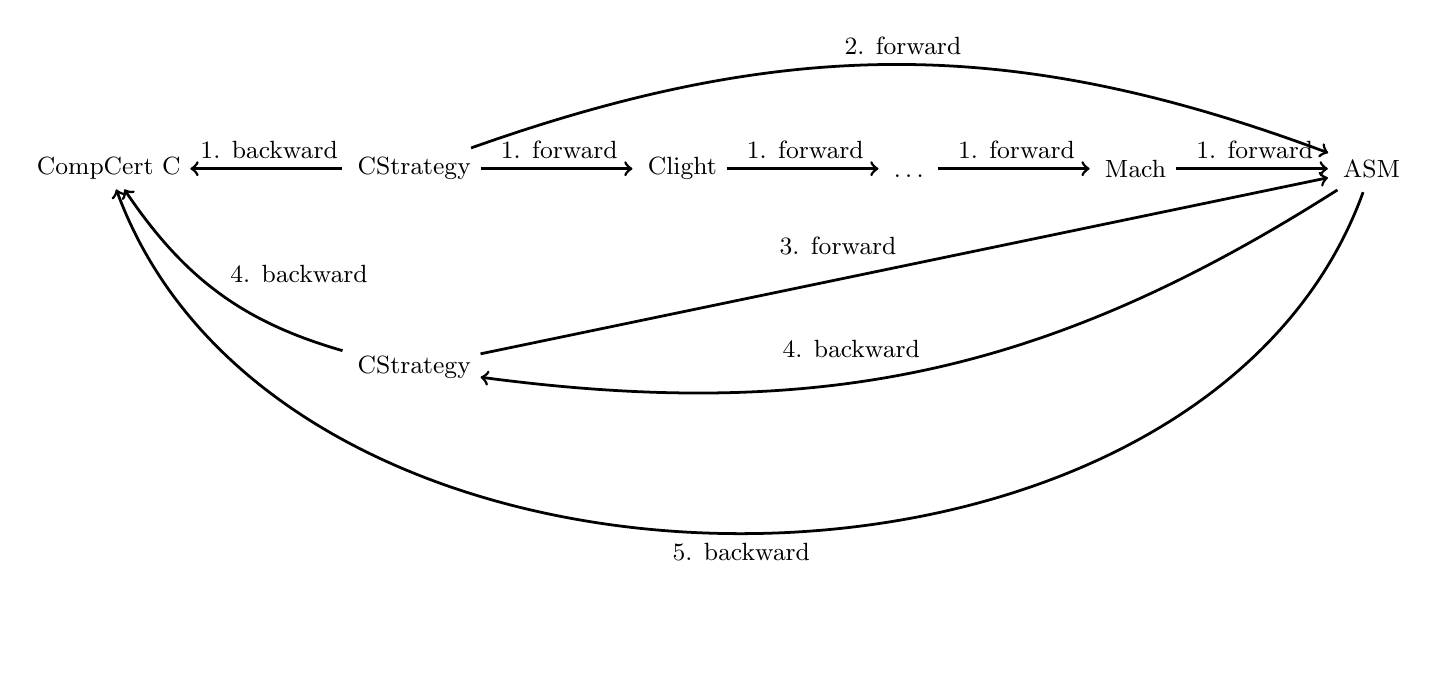
\begin{tikzpicture}[%
        every node/.style={rectangle, font=\small},
        shorten >=2pt,
        node distance=2cm
      ]
      \node (cc) {CompCert C};
      \node (cstrat) [right=of cc] {CStrategy};
      \node (clight) [right=of cstrat] {Clight};
      \node (dots) [right=of clight] {\dots\vphantom{C}};
      \node (mach) [right=of dots] {Mach};
      \node (asm) [right=of mach] {ASM};
      \node (atcstrat) [below=of cstrat] {\at{CStrategy}};
      \path [draw] (cc) edge[<-, above,line width=1pt] node {1. backward} (cstrat);
      \path [draw] (cstrat) edge[->, above,line width=1pt] node {1. forward} (clight);
      \path [draw] (clight) edge[->, above,line width=1pt] node {1. forward} (dots);
      \path [draw] (dots) edge[->, above,line width=1pt] node {1. forward} (mach);
      \path [draw] (mach) edge[->, above,line width=1pt] node {1. forward} (asm);
      \path [draw] (cstrat) edge[->, bend left=20, above,line width=1pt] node {2. forward} (asm);
      \path [draw] (atcstrat) edge[->, above left,line width=1pt] node {3. forward} (asm);
      \path [draw] (cc) edge[<-, bend right=20, above right,line width=1pt] node {4. backward} (atcstrat);
      \path [draw] (atcstrat) edge[<-, bend right=20, above left,line width=1pt] node {4. backward} (asm);
      \path [draw] (cc) edge[<-, bend right=70, below,line width=1pt] node {5. backward} (asm);
    \end{tikzpicture}
}

\subsubsection{Theorem: Factor forward simulation} If there is a forward simulation between $S_1$ and $S_2$ and $S_2$ has \textit{single events}, then there is a forward simulation between $\mathit{Atomic}(S_1)$ and $S_2$.

\subsubsection{Correctness proof}
The previous proof in CompCert used the following reasoning:
\begin{enumerate}
\item Prove a forward simulation for each pass between CStrategy and ASM. Prove a backward simulation between CompCert C and Cstrategy.
\item Use the simulation composition theorem to deduce a forward simulation between CStrategy and ASM
\item Use the Factor forward simulation theorem to deduce a forward simulation between $\mathit{Atomic}(\text{CStrategy})$ and ASM.
\item Use the forward to backward theorem to deduce a backward simulation between $\mathit{Atomic}(\text{CStrategy})$ and ASM, as well as the factor backward theorem to deduce a backward simulation between CompCert C and $\mathit{Atomic}(\text{CStrategy})$.
\item Use the simulation composition theorem to deduce a backward simulation between CompCert C and ASM.
\end{enumerate}

This proof is illustrated Figure~\ref{fig:oldproof}.

\begin{figure}
  \makebox[\textwidth][c]{\oldproof}
  \caption{The previous correctness proof}
  \label{fig:oldproof}
\end{figure}


\end{document}
